\chapter{Applications}
\label{chap:applications}

Having investigated the theoretical properties of our method, it remains to empirically assess its performance. For the first test scenario, we have selected the Lotka-Volterra model described in \autoref{sec:lotka-volterra}. This is a relatively simple problem whose purpose is to validate our conclusions from the theoretical analysis. The second example is a simplified model for a prokaryotic auto-regulatory network addressed in \autoref{sec:autoregulation}. In both scenarios, the particle filter-based approach is compared with our ABC approximation under various model misspecifications.

The considered problems require simulating stochastic reactions in order to propagate the system states through time. This is done with the help of the Gillespie algorithm, which is first described in \autoref{sec:gillespie}.


\section{Implementation notes}
All of the experiments described below have been implemented in Python 3.6.5. The performance-critical parts were additionally written in Cython to obtain C-like performance. The only additional dependencies are NumPy 1.14.3, SciPy 1.2.1, Matplotlib 2.2.2 and Statsmodels 0.9.0. The experiments have been performed on a standard laptop computer.


\section{Preliminary: the Gillespie algorithm} \label{sec:gillespie}
The Gillespie algorithm \citep{gillespie1, gillespie2} is used to simulate a stochastic process describing the time evolution of a system of reactions. The discussion given here follows \cite{wilkinson-book}.

\paragraph{Time evolution of a reaction system}
Consider a system consisting of $u$ species $\mathcal{X}_1, \ldots, \mathcal{X}_u$ and $v$ reactions $\mathcal{R}_1, \ldots, \mathcal{R}_v$. The species can describe literal animal species, as is the case in the Lotka-Volterra model in \autoref{sec:lotka-volterra}, or individual molecule types, as in \autoref{sec:autoregulation}. The reactions describe the interactions between these species through time.

Let the number of molecules (or individuals, in case of animal species) of the species $\mathcal{X}_i$ at time $t$ be denoted by $X_{i,t}$, and let $\bm{X}_t = \left(X_{1,t}, \ldots, X_{u,t}\right)^\intercal$. Additionally, let the number of reactions of type $\mathcal{R}_i$ which occurred in a time window $(0, t]$ be denoted by $R_{i,t}$, and let $\bm{R}_t = \left(R_{1,t}, \ldots,R_{v,t}\right)^\intercal$. The evolution of the system from time 0 to time $t$ is described by the equation
\begin{equation} \label{eq:system-evolution}
\bm{X}_t - \bm{X}_0 = \mathbb{S}\bm{R}_t,
\end{equation}
where $\mathbb{S} \in \R^{u \times v}$ is called the stoichiometry matrix of the system, and describes the difference in the number of molecules of each species after each reaction occurs. To gain insight into the meaning of $\mathbb{S}$, it is instructive to write it as
\begin{equation*}
\mathbb{S} = \mathbb{P}_\text{post} - \mathbb{P}_\text{pre},
\end{equation*}
where the element $(i,j)$ of $\mathbb{P}_\text{pre}$ denotes the number of molecules of $\mathcal{X}_i$ before a reaction of type $\mathcal{R}_j$ takes place, and the element $(i,j)$ of $\mathbb{P}_\text{post}$ describes the same quantity \emph{after} it takes place. Equation \eqref{eq:system-evolution} can then be written as
\begin{equation*}
\bm{X}_t = \bm{X}_0 + \left(\mathbb{P}_\text{post} - \mathbb{P}_\text{pre}\right) \bm{R}_t,
\end{equation*}
and describes the net gain in the number of molecules of each species given their initial numbers, and accounting for their increase/decrease when a number of reactions of each type occurs.

In addition, each reaction $\mathcal{R}_i$ has a stochastic rate constant $c_i$ and a rate law (also called the hazard function) $h_i(\bm{X}_t, c_i)$ associated with it. The interpretation of the hazard function is such that $h_i(\bm{X}_t, c_i) \dx{t}$ is the probability of a reaction of type $\mathcal{R}_i$ occurring in a time interval $(t, t + \dx{t}]$, conditionally on the system being in state $\bm{X}_t$. Such a situation is described by an exponential distribution -- the time to the event of a reaction of type $\mathcal{R}_i$ occurring, assuming no other reaction is taking place, is distributed according to ${\mathcal{E}\mathit{xp}\left(h_i(\bm{X}_t, c_i)\right)}$. This is however a convenient simplification, since multiple reactions are typically occurring at the same time.

\paragraph{The Gillespie algorithm}
In a system with $v$ reactions and their hazard functions $h_i(\bm{X}_t, c_i)$, the hazard of \emph{some} reaction occurring is
\begin{equation*}
h_0(\bm{X}_t, \bm{c}) = \sum_{i=0}^v h_i(\bm{X}_t, c_i),
\end{equation*}
where $\bm{c} = \left(c_1, \ldots, c_v\right)^\intercal$. The time to the next reaction is then distributed according to $\mathcal{E}\mathit{xp}\left(h_0(\bm{X}_t, \bm{c})\right)$. The particular reaction type is a random variable with a categorical distribution $\mathcal{C}\mathit{at}\left(\widetilde{h}_1(\bm{X}_t,c_1), \ldots, \widetilde{h}_v(\bm{X}_t,c_v)\right)$, where $\displaystyle \widetilde{h}_i(\bm{X}_t,c_i) = \frac{h_i(\bm{X}_t,c_i)}{h_0(\bm{X}_t, \bm{c})}$.

With the above in mind, the Gillespie algorithm can now be formulated, and is given in \autoref{alg:gillespie}. Its purpose is to simulate the state evolution \eqref{eq:system-evolution} for a given time horizon $T$ while accounting for the randomness in the time until a reaction of a particular type takes place. For the purpose of this algorithm, denote the columns of the stoichiometry matrix $\mathbb{S}$ by $\bm{S}^i, \quad i = 1, \ldots, v$.
\begin{algorithm}[ht]
    \caption{Gillespie algorithm}
    \label{alg:gillespie}
    \begin{algorithmic}[1]
        \Input $\text{Time horizon } T, \text{ rate constants } \bm{c} = \left(c_1, \ldots, c_v\right)^\intercal,\ \text{initial molecule numbers } \bm{X}_0.$
        
        \State $t \gets 0$
        
        \State $\bm{X}_t \gets \bm{X}_0$
        
        \While{$t \leq T$}
            \State $\text{Calculate } h_i(\bm{X}_t, c_i), \quad i = 1, \ldots, v.$
            \State $h_0(\bm{X}_t, \bm{c}) \gets \sum_{i=1}^v h_i(\bm{X}_t, c_i)$
            \State $\text{Calculate } \displaystyle \widetilde{h}_i(\bm{X}_t,c_i) = \frac{h_i(\bm{X}_t,c_i)}{h_0(\bm{X}_t, \bm{c})}, \quad i = 1, \ldots, v.$
            \State $\text{Sample } \dx{t} \sim \mathcal{E}\mathit{xp}\left(h_0(\bm{X}_t, \bm{c})\right).$ \Comment{Simulate the time to the next reaction.}
            \State $\text{Sample } i \sim \mathcal{C}\mathit{at}\left(\widetilde{h}_1(\bm{X}_t,c_1), \ldots, \widetilde{h}_v(\bm{X}_t,c_v)\right).$ \Comment{Simulate the reaction type.}
            \State $\bm{X}_{t + \dx{t}} \gets \bm{X}_t + \bm{S}^i$ \Comment{Update the state according to the reaction $i$.}
            \State $t \gets t + \dx{t}$
        \EndWhile
        
        \Output $\text{Final state } \bm{X}_t, \text { final time } t.$
    \end{algorithmic}
\end{algorithm}

The algorithm is usually the bottleneck of most simulations, and must be implemented carefully; otherwise, the simulation becomes unacceptably slow. The final time $t$ is at the output as well, since it may exceed the horizon $T$. If the algorithm is run consecutively during a simulation, the interest is to follow the previous run by starting at its final time $t$.

\section{Lotka-Volterra model} \label{sec:lotka-volterra}
\subsection{Problem description}
The first considered problem is the Lotka-Volterra model \citep{lotka, volterra}. The system describes a simplified time interaction of a population consisting of a predator and prey species. Denoting the prey species by $\mathcal{X}_1$ and the predator species by $\mathcal{X}_2$, the system can be described by the reactions
\begin{align}
\mathcal{R}_1:\quad & \mathcal{X}_1 \to 2 \mathcal{X}_1, \label{eq:lv1} \\
\mathcal{R}_2:\quad & \mathcal{X}_1 + \mathcal{X}_2 \to 2 \mathcal{X}_2, \label{eq:lv2} \\
\mathcal{R}_3:\quad & \mathcal{X}_2 \to \emptyset. \label{eq:lv3}
\end{align}
Equation \eqref{eq:lv1} describes the reproduction of the prey species. Equation \eqref{eq:lv2} describes the interaction between the predator and the prey where a predator consumes an individual of the prey species and produces an offspring. Equation \eqref{eq:lv3} describes the extinction of the predator species when no prey is present.

The state of the system at time $t$ is $\bm{X}_t = \left(X_{1,t}, X_{2,t}\right)^\intercal$. The stoichiometry matrix is given by
\begin{equation*}
\mathbb{S} = \begin{pmatrix}
1 & -1 & 0 \\
0 & 1 & -1 \\
\end{pmatrix},
\end{equation*}
and the hazard functions vector is $\bm{h}(\bm{X}, \bm{c}) = \left(c_1 X_{1}, c_2 X_{1} X_{2}, c_3 X_{2}\right)^\intercal$ \citep{wilkinson}. Although simple to describe, this model is analytically intractable \citep{wilkinson-book}.

For the inference problem, we consider the unknown parameters to be $\btheta = \left(c_1, c_2, c_3\right)^\intercal$, and the state at time $t$ to be $\bx_t = \left(X_{1,t}, X_{2,t}\right)^\intercal$. Since the rate constants $c_1, c_2, c_3$ are by definition positive, we are working in the log space to avoid restricting ourselves to positive support distributions. The model is specified by the following:
\begin{equation*}
\begin{split}
\sprior(x_{1,0} \mid \btheta) &= \mathcal{P}\mathit{o}\left(50\right), \\
\sprior(x_{2,0} \mid \btheta) &= \mathcal{P}\mathit{o}\left(100\right), \\
\trans_t(\bx_t \mid \bx_{t-1}, \btheta) & \text{ is simulated using \autoref{alg:gillespie} }, \\
\obs_t(\by_t \mid \bx_{t}, \btheta) &= \mathcal{N}_2\left(\bx_t, 10^2\right).
\end{split}
\end{equation*}
The parameter prior and the Metropolis-Hastings proposal are additionally given by
\begin{equation*}
\begin{split}
\pprior(\log c_i) &= \mathcal{U}\left(-7, 2\right), \quad i = 1, 2, 3, \\
\prop(\btheta^\prime \mid \btheta) &= \mathcal{N}_3\left(\btheta, 0.01 \mathbb{I}_3\right).
\end{split}
\end{equation*}
The initial parameters are $\btheta^{(0)} = \left(1, 0.005, 0.6\right)^\intercal$. We simulate a sequence of 16 observations $\by_t$ using the Gillespie algorithm with parameters $\btheta^{(0)}$. The inference is started in the correct parameters and applied on a short sequence only; its purpose is only to demonstrate that the algorithm is able to identify these parameters.

We apply the marginal Metropolis-Hastings algorithm depending on the particle filter as well as the one utilizing ABC methods. Both algorithms are ran for $M = 50000$ samples with $N = 100$ particles. Additionally, the number of covered pseudo-observations in the ABC formulation is $\alpha = 90$ and the volume of the p-HPR is $p = 0.95$.

When using the ABC method, we simulate pseudo-observations from the observation model $\obs_t$ without the noise term. That is, we simulate $\bu_t = \bx_t$, deterministically.

\subsection{Inference using the particle filter}
To start, we consider inference using \autoref{alg:marginal-metropolis-hastings}, i.e., using the particle filter to approximate the likelihood.

\paragraph{Correctly specified observation model}
At first, we assume the correct model specification. This means that the observations $\by_t$ have been corrupted by Gaussian noise, and the observation model $\obs_t$ is Gaussian as well. In this situation, the particle filter is expected to perform well, as all assumptions have been met.

In \autoref{fig:lv-pmh-gauss-c1}, \autoref{fig:lv-pmh-gauss-c2} and \autoref{fig:lv-pmh-gauss-c3}, the results for the parameters $c_1$, $c_2$ and $c_3$, respectively, are shown. For each parameter, we show (in this order) the trace plot, the autocorrelation plot, and the histogram of sampled values. We use no burn-in period, as the inference starts in the correct values, but apply thinning of 100, i.e., keep every 100th sample. This ensures relatively uncorrelated samples, as is clear from the auto-correlation plots. The acceptation rate of the Metropolis-Hastings algorithms moves around 20 \%.

\begin{figure}[htp]
    \centering
    \includegraphics[width=0.7\linewidth]{lotka-volterra/pmh_gauss_c1}
    \caption{Particle filter-based inference of the parameter $c_1$ in the Lotka-Volterra model. Uses Gaussian noise and a Gaussian observation model. The true value is shown in red.}
    \label{fig:lv-pmh-gauss-c1}
\end{figure}

\begin{figure}[htp]
    \centering
    \includegraphics[width=0.7\linewidth]{lotka-volterra/pmh_gauss_c2}
    \caption{Particle filter-based inference of the parameter $c_2$ in the Lotka-Volterra model. Uses Gaussian noise and a Gaussian observation model. The true value is shown in red.}
    \label{fig:lv-pmh-gauss-c2}
\end{figure}

\begin{figure}[htp]
    \centering
    \includegraphics[width=0.7\linewidth]{lotka-volterra/pmh_gauss_c3}
    \caption{Particle filter-based inference of the parameter $c_3$ in the Lotka-Volterra model. Uses Gaussian noise and a Gaussian observation model. The true value is shown in red.}
    \label{fig:lv-pmh-gauss-c3}
\end{figure}

In all cases, the correct parameters are well-covered by the sampled values, while allowing for some degree of variance. The histograms provide estimated posterior distributions of the individual parameters. The sampled values can be used to provide point estimates or credible intervals for the true parameters.

\paragraph{Misspecified observation model}
Next, we keep the Gaussian observation model, but corrupt the observation sequence by a Cauchy noise with scale 10. Arguably, this scale is quite high, but is used to match the scale of the Gaussian noise from the previous section. The heavy-tailed Cauchy distribution allows sampling distant noise terms, and corrupts the observation sequence $\by_t$ much more severely. The Gaussian observation model $\obs_t$ then assigns probability close to zero to these values, and the filter collapses. This is clear from \autoref{fig:lv-pmh-cauchy-c1}, \autoref{fig:lv-pmh-cauchy-c2} and \autoref{fig:lv-pmh-cauchy-c3}.

\begin{figure}[htp]
    \centering
    \includegraphics[width=0.7\linewidth]{lotka-volterra/pmh_cauchy_c1}
    \caption{Particle filter-based inference of the parameter $c_1$ in the Lotka-Volterra model. Uses Cauchy noise and a Gaussian observation model. The true value is shown in red.}
    \label{fig:lv-pmh-cauchy-c1}
\end{figure}

\begin{figure}[htp]
    \centering
    \includegraphics[width=0.7\linewidth]{lotka-volterra/pmh_cauchy_c2}
    \caption{Particle filter-based inference of the parameter $c_2$ in the Lotka-Volterra model. Uses Cauchy noise and a Gaussian observation model. The true value is shown in red.}
    \label{fig:lv-pmh-cauchy-c2}
\end{figure}

\begin{figure}[htp]
    \centering
    \includegraphics[width=0.7\linewidth]{lotka-volterra/pmh_cauchy_c3}
    \caption{Particle filter-based inference of the parameter $c_3$ in the Lotka-Volterra model. Uses Cauchy noise and a Gaussian observation model. The true value is shown in red.}
    \label{fig:lv-pmh-cauchy-c3}
\end{figure}

Clearly, Cauchy noise corrupts the sequence too much, and the results are poor. The accepted parameters are almost constant, and the posterior distribution is not even remotely-well approximated. This is an expected behavior, since the particle filter is known not to perform well under model misspecification.



\subsection{Inference using ABC}
Next, we apply \autoref{alg:marginal-metropolis-hastings-abc}, the variant of the Metropolis-Hastings algorithm depending on ABC.

\paragraph{Gaussian noise, Gaussian kernel}
At first, we again corrupt the sequence $\by_t$ by a Gaussian noise, as indicated above. We then run \autoref{alg:marginal-metropolis-hastings-abc} with a Gaussian kernel to infer about the parameters $\btheta$. The results are shown in \autoref{fig:lv-abcmh-gauss-gauss-c1}, \autoref{fig:lv-abcmh-gauss-gauss-c2} and \autoref{fig:lv-abcmh-gauss-gauss-c3}.

\begin{figure}[htp]
    \centering
    \includegraphics[width=0.7\linewidth]{lotka-volterra/abcmh_gauss_gauss_c1}
    \caption{ABC-based inference of the parameter $c_1$ in the Lotka-Volterra model. Uses Gaussian noise and a Gaussian kernel. The true value is shown in red.}
    \label{fig:lv-abcmh-gauss-gauss-c1}
\end{figure}

\begin{figure}[htp]
    \centering
    \includegraphics[width=0.7\linewidth]{lotka-volterra/abcmh_gauss_gauss_c2}
    \caption{ABC-based inference of the parameter $c_2$ in the Lotka-Volterra model. Uses Gaussian noise and a Gaussian kernel. The true value is shown in red.}
    \label{fig:lv-abcmh-gauss-gauss-c2}
\end{figure}

\begin{figure}[htp]
    \centering
    \includegraphics[width=0.7\linewidth]{lotka-volterra/abcmh_gauss_gauss_c3}
    \caption{ABC-based inference of the parameter $c_3$ in the Lotka-Volterra model. Uses Gaussian noise and a Gaussian kernel. The true value is shown in red.}
    \label{fig:lv-abcmh-gauss-gauss-c3}
\end{figure}

Compared to the results obtained by running the particle filter-based inference with a correct observation model, the results are slightly worse in the case of $c_1$, as the true value is in a region with a lower probability. Somewhat worse result is to be expected though, since the ABC methods provide only an approximation. Otherwise, the results are comparable to those utilizing the particle filter.


\paragraph{Cauchy noise, Gaussian kernel}
Next, we again corrupt the observation sequence by the heavy-tailed Cauchy noise. First, we keep the Gaussian kernel to calculate the importance weights. The results are in \autoref{fig:lv-abcmh-cauchy-gauss-c1}, \autoref{fig:lv-abcmh-cauchy-gauss-c2} and \autoref{fig:lv-abcmh-cauchy-gauss-c3}.

Compared to the particle filter with a misspecified observation model, the filter does not collapse at all. Instead, it remains stable, and the results resemble those obtained from a particle filter assuming a correct observation model, or those given by the previous ABC use-case.

This shows the strength of the ABC approximation -- even under a heavy-tailed noise such as the Cauchy one, using a set of simulated pseudo-observations with a suitable kernel function allows the likelihood estimate to remain stable even under a severe model misspecification.

\begin{figure}[htp]
    \centering
    \includegraphics[width=0.7\linewidth]{lotka-volterra/abcmh_cauchy_gauss_c1}
    \caption{ABC-based inference of the parameter $c_1$ in the Lotka-Volterra model. Uses Cauchy noise and a Gaussian kernel. The true value is shown in red.}
    \label{fig:lv-abcmh-cauchy-gauss-c1}
\end{figure}

\begin{figure}[htp]
    \centering
    \includegraphics[width=0.7\linewidth]{lotka-volterra/abcmh_cauchy_gauss_c2}
    \caption{ABC-based inference of the parameter $c_2$ in the Lotka-Volterra model. Uses Cauchy noise and a Gaussian kernel. The true value is shown in red.}
    \label{fig:lv-abcmh-cauchy-gauss-c2}
\end{figure}

\begin{figure}[htp]
    \centering
    \includegraphics[width=0.7\linewidth]{lotka-volterra/abcmh_cauchy_gauss_c3}
    \caption{ABC-based inference of the parameter $c_3$ in the Lotka-Volterra model. Uses Cauchy noise and a Gaussian kernel. The true value is shown in red.}
    \label{fig:lv-abcmh-cauchy-gauss-c3}
\end{figure}

\paragraph{Cauchy noise, Cauchy kernel}
Finally, we repeat the same experiment as in the previous section, but use a Cauchy kernel instead of the Gaussian one. The results are very similar to those obtained using a Gaussian kernel, indicating that the filter is fairly robust to kernel choice. This agrees with the conclusion provided by \cite{dedecius}.

The Cauchy kernel might be preferable to the Gaussian one for computational reasons -- its quantile function (required for kernel width tuning) can be calculated without resorting to numerical approximations.

\begin{figure}[ht]
    \centering
    \includegraphics[width=0.7\linewidth]{lotka-volterra/abcmh_cauchy_cauchy_c1}
    \caption{ABC-based inference of the parameter $c_1$ in the Lotka-Volterra model. Uses Cauchy noise and a Cauchy kernel. The true value is shown in red.}
    \label{fig:lv-abcmh-cauchy-cauchy-c1}
\end{figure}

\begin{figure}[ht]
    \centering
    \includegraphics[width=0.7\linewidth]{lotka-volterra/abcmh_cauchy_cauchy_c2}
    \caption{ABC-based inference of the parameter $c_2$ in the Lotka-Volterra model. Uses Cauchy noise and a Cauchy kernel. The true value is shown in red.}
    \label{fig:lv-abcmh-cauchy-cauchy-c2}
\end{figure}

\begin{figure}[ht]
    \centering
    \includegraphics[width=0.7\linewidth]{lotka-volterra/abcmh_cauchy_cauchy_c3}
    \caption{ABC-based inference of the parameter $c_3$ in the Lotka-Volterra model. Uses Cauchy noise and a Cauchy kernel. The true value is shown in red.}
    \label{fig:lv-abcmh-cauchy-cauchy-c3}
\end{figure}


\subsection{Experiment conclusion}
The Lotka-Volterra simulation study demonstrated the performance of our algorithm and confirmed our expectations about the differences between the particle filter and our ABC-based method. As indicated in \autoref{chap:inference}, the particle filter-based inference using the correct observation model gives the best results. The sampled values well cover the true parameter and have a reasonable degree of variance. On the other hand, when the observation model is misspecified, the filter completely collapses, and the inference becomes unreliable.

Application of the ABC framework to the correctly specified model introduces some bias which was theoretically justified in \autoref{chap:abc}. The method achieves a slightly worse precision than the particle filter, although the results are still sensible. ABC mainly excels under a misspecified model and prevents the filter from collapsing, while still achieving results comparable to the correctly parameterized particle filter. In addition, the ABC filter is not particularly sensitive to the kernel choice. These points make our method a superior choice when the true observation model is not known, as it allows for stable inference at a similar computational cost.



\section{Prokaryotic auto-regulation model} \label{sec:autoregulation}
\subsection{Problem description}
The second considered model comes from \cite{wilkinson2, wilkinson}, and describes a simplified prokaryotic autoregulatory gene network. The discussion below follows these two papers.

The model assumes that the dimer of a protein $P$, denoted $P_2$, represses the transcription of its coding gene by binding to a regulatory region in the gene. This transcription begins by binding of RNA-polymerase to the promoter of the gene. As the RNA-polymerase moves along the gene, it transcripts the gene into mRNA. The transcription is repressed by binding of $P_2$ to regions od the gene called operators. The repression and transcription can be described in a simplified way by the following reactions:
\begin{equation*}
\begin{split}
\mathcal{R}_1:\quad & \mathit{DNA} + P_2 \to \mathit{DNA} \cdot P_2 \\
\mathcal{R}_2:\quad & \mathit{DNA} \cdot P_2 \to \mathit{DNA} + P_2 \\
\mathcal{R}_3:\quad & \mathit{DNA} \to \mathit{DNA} + \mathit{RNA}.
\end{split}
\end{equation*}

The entire process of translating the mRNA into the protein $P$ is summarized by the single reaction
\begin{equation*}
\mathcal{R}_4:\quad \mathit{RNA} \to \mathit{RNA} + P.
\end{equation*}

The reversible dimerization of $P$ is described by
\begin{equation*}
\begin{split}
\mathcal{R}_5:\quad & 2P \to P_2 \\
\mathcal{R}_6:\quad & P_2 \to 2P.
\end{split}
\end{equation*}

The remaining two reactions describe mRNA and protein degradation
\begin{equation*}
\begin{split}
\mathcal{R}_7:\quad & \mathit{RNA} \to \emptyset \\
\mathcal{R}_8:\quad & P \to \emptyset.
\end{split}
\end{equation*}

The state of the system at time $t$ is $\bm{X}_t = \left(\mathit{RNA}_t, P_t, (P_2)_t, (\mathit{DNA} \cdot P_2)_t, \mathit{DNA}_t\right)^\intercal$. The stoichiometry matrix is given by
\begin{equation} \label{eq:singular-stoichiometry}
\mathbb{S} = \begin{pmatrix}
0 & 0 & 1 & 0 & 0 & 0 & -1 & 0 \\
0 & 0 & 0 & 1 & -2 & 2 & 0 & -1 \\
-1 & 1 & 0 & 0 & 1 & -1 & 0 & 0 \\
1 & -1 & 0 & 0 & 0 & 0 & 0 & 0 \\
-1 & 1 & 0 & 0 & 0 & 0 & 0 & 0
\end{pmatrix},
\end{equation}
and the hazard function vector is \citep{wilkinson}
\begin{equation*}
\bm{h}(\bm{X}, \bm{c}) = \left(c_1 P_2 \mathit{DNA}, c_2 \mathit{DNA} \cdot P_2, c_3 \mathit{DNA}, c_4 \mathit{RNA}, \frac{c_5 P(P-1)}{2}, c_6 P_2, c_7 \mathit{RNA}, c_8 P \right)^\intercal.
\end{equation*}

The matrix \eqref{eq:singular-stoichiometry} is singular, as we can add the last two rows together to produce a zero vector. Given the variable ordering in $\bm{X}_t$, this implies that
\begin{equation*}
\mathit{DNA} \cdot P_2 + \mathit{DNA} = k,
\end{equation*}
where $k$ is a constant. This is equation is called a conservation law, and the constant $k$ denotes the number of copies of the particular gene in the genome. From this conservation law, it follows that $\mathit{DNA} \cdot P_2 = k - \mathit{DNA}$, which we substitute into the system described above. This results in a system of four variables only, denoted ${\bm{X}_t = \left(\mathit{RNA}_t, P_t, (P_2)_t, \mathit{DNA}_t\right)^\intercal}$.

This substitution simplifies the stoichiometry matrix \eqref{eq:singular-stoichiometry} into
\begin{equation*}
\mathbb{S} = \begin{pmatrix}
0 & 0 & 1 & 0 & 0 & 0 & -1 & 0 \\
0 & 0 & 0 & 1 & -2 & 2 & 0 & -1 \\
-1 & 1 & 0 & 0 & 1 & -1 & 0 & 0 \\
-1 & 1 & 0 & 0 & 0 & 0 & 0 & 0
\end{pmatrix},
\end{equation*}
and the hazard function vector into
\begin{equation*}
\bm{h}(\bm{X}, \bm{c}) = \left(c_1 P_2 \mathit{DNA}, c_2 (k - \mathit{DNA}), c_3 \mathit{DNA}, c_4 \mathit{RNA}, \frac{c_5 P(P-1)}{2}, c_6 P_2, c_7 \mathit{RNA}, c_8 P \right)^\intercal.
\end{equation*}

For the inference problem, the unknown parameters are $\btheta = \left(c_1, c_2, c_3, c_4, c_7, c_8\right)^\intercal$. The parameters $c_5$ and $c_6$ are assumed to be known, exactly as in \cite{wilkinson}. The latent state at time $t$ is $\bx_t = \left(\mathit{RNA}_t, P_t, (P_2)_t, \mathit{DNA}_t\right)^\intercal$. We again work in the log-space, as the rate constants are positive by definition. The model described by \cite{wilkinson} assumes the initial state to be known $\bx_0 = \left(8,8,8,5\right)^\intercal$, ${k = 10}$, ${c_5 = 0.1}$, ${c_6 = 0.9}$, and that
\begin{equation*}
\begin{split}
\trans_t(\bx_t \mid \bx_{t-1}, \btheta) & \text{ is simulated using \autoref{alg:gillespie} }, \\
\obs_t(\by_t \mid \bx_{t}, \btheta) &= \mathcal{N}\left(P_t + 2 (P_2)_t, 2^2\right).
\end{split}
\end{equation*}
This means we are only able to observe the protein concentrations, subject to error. The problem becomes considerably more challenging compared to the Lotka-Volterra model, where we observed the entire state vector (up to noise). Here we only observe a noisy linear combination of two elements of the latent state, which makes the inference much more difficult. The biological interpretation is that we are not able to distinguish the protein monomers from its dimers.

The parameter prior and the Metropolis-Hastings proposal are additionally given by
\begin{equation*}
\begin{split}
\pprior(\log c_i) &= \mathcal{U}\left(-7, 2\right), \quad i = 1, 2, 3, 4, 7, 8, \\
\prop(\btheta^\prime \mid \btheta) &= \mathcal{N}_6\left(\btheta, 0.08 \mathbb{I}_6\right).
\end{split}
\end{equation*}
The initial parameters are sampled from the prior distributions. We simulate the data $\by_t$ using \autoref{alg:gillespie} and obtain a sequence of $T = 237$ observations $\by_t \sim \mathcal{N}\left(P_t + 2 (P_2)_t, 2^2\right)$.

The marginal Metropolis-Hastings is run again for $M = 50000$ samples, this time with $N = 200$ particles. We use a burn-in period of 10000 and thin the samples by 25. The ABC parameters are $\alpha = 180$ and $p = 0.95$. The pseudo-observations are again simulated from $\obs_t$ without the noise term.

\subsection{Inference using the particle filter}
We again start by applying the particle filter-based algorithm. At first, we examine the results under a well-specified model. Next, we use a misspecified model by once again corrupting the input sequence by the Cauchy noise.

\paragraph{Correctly specified observation model}
At first, we consider the model exactly as described above, and perform inference using the particle filter. This is a well-specified model, since the observation model $\obs_t$ coincides with the noise on the data sequence $\by_{1:T}$. The results are shown in \autoref{fig:ar-pmh-gauss-1}, \autoref{fig:ar-pmh-gauss-2} and \autoref{fig:ar-pmh-gauss-3}.

Most of the parameters (apart from $c_4$) are well-covered by the posterior samples, agreeing with the results of \cite{wilkinson}. Even after thinning, we see that the samples are highly correlated. The original authors did not provide any autocorrelation plots, so the results cannot be compared. Having such correlated samples means that calculating empirical estimates would be unreliable, as they typically require independent observations. This issue could be addressed by considering more complex proposal distributions or samplers.

\begin{figure}[htp]%
    \centering
    \subfloat[$c_1$]{{\includegraphics[width=0.45\textwidth]{autoregulation/pmh_gauss_c1} }}%
    \qquad
    \subfloat[$c_2$]{{\includegraphics[width=0.45\textwidth]{autoregulation/pmh_gauss_c2} }}%
    \caption{Particle filter-based inference of the parameters $c_1$ and $c_2$ in the auto-regulation model. Uses Gaussian noise and a Gaussian observation model. The true values are shown in red.}%
    \label{fig:ar-pmh-gauss-1}%
\end{figure}

\begin{figure}[htp]%
    \centering
    \subfloat[$c_3$]{{\includegraphics[width=0.45\textwidth]{autoregulation/pmh_gauss_c3} }}%
    \qquad
    \subfloat[$c_4$]{{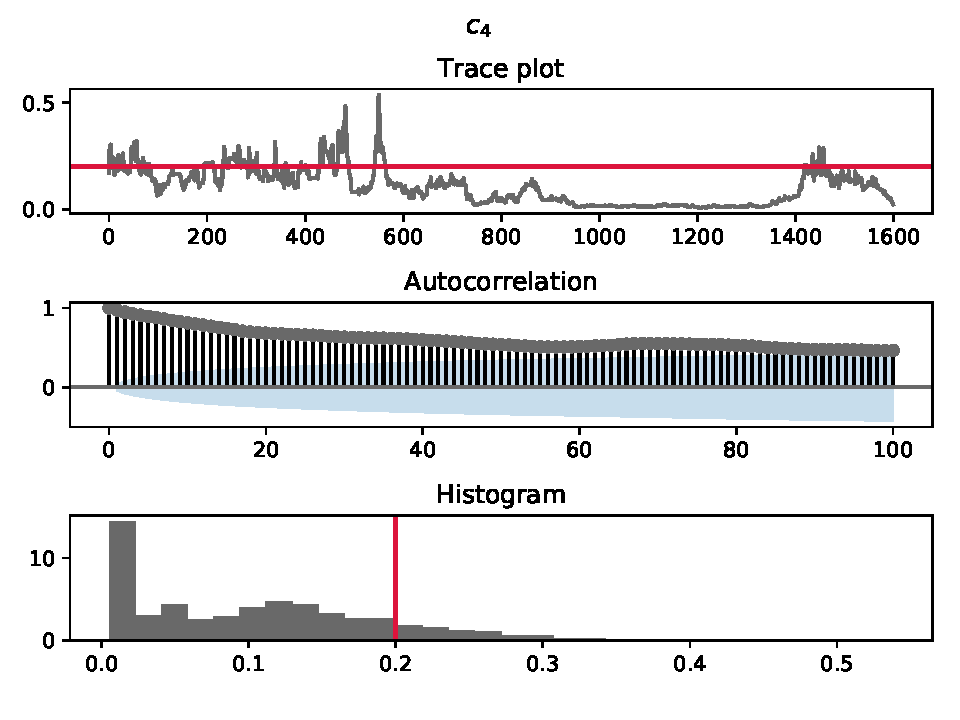
\includegraphics[width=0.45\textwidth]{autoregulation/pmh_gauss_c4} }}%
    \caption{Particle filter-based inference of the parameters $c_3$ and $c_4$ in the auto-regulation model. Uses Gaussian noise and a Gaussian observation model. The true values are shown in red.}%
    \label{fig:ar-pmh-gauss-2}%
\end{figure}

\begin{figure}[htp]%
    \centering
    \subfloat[$c_7$]{{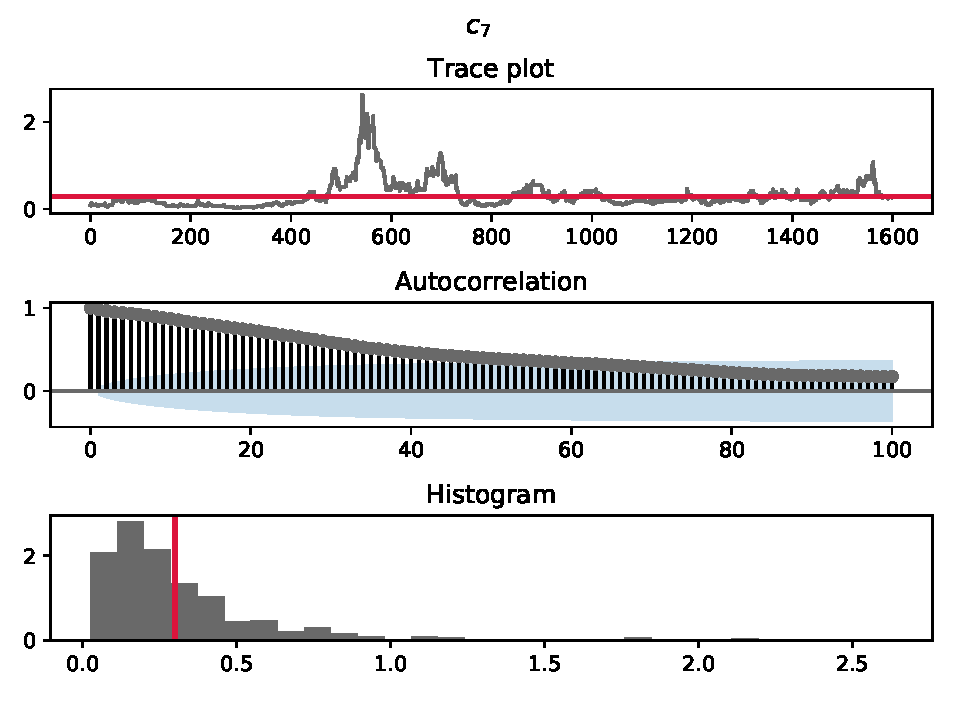
\includegraphics[width=0.45\textwidth]{autoregulation/pmh_gauss_c7} }}%
    \qquad
    \subfloat[$c_8$]{{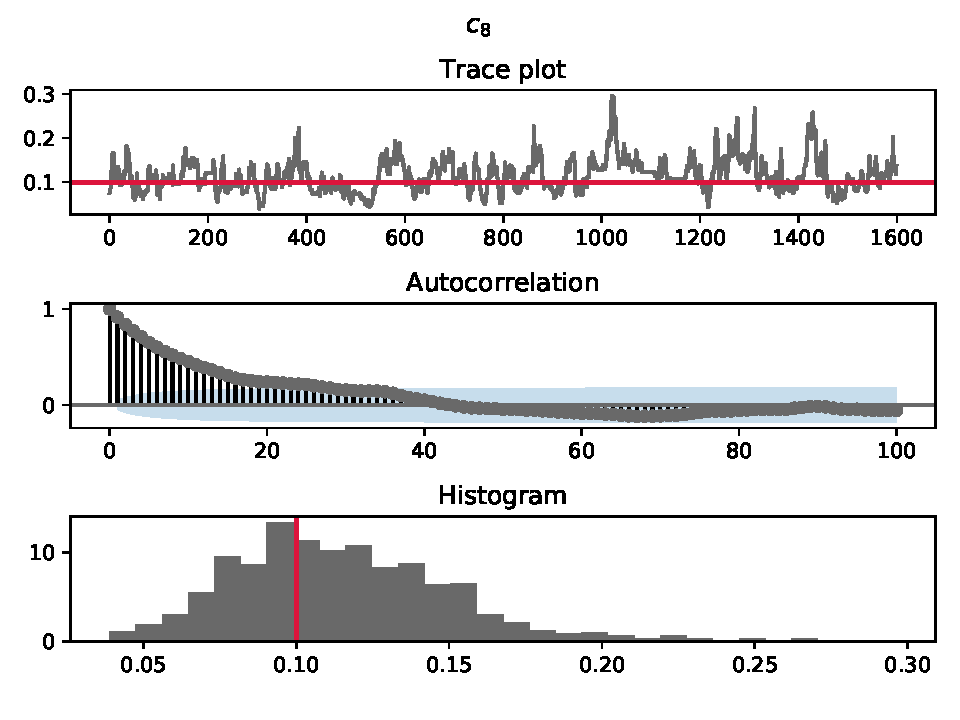
\includegraphics[width=0.45\textwidth]{autoregulation/pmh_gauss_c8} }}%
    \caption{Particle filter-based inference of the parameters $c_7$ and $c_8$ in the auto-regulation model. Uses Gaussian noise and a Gaussian observation model. The true values are shown in red.}%
    \label{fig:ar-pmh-gauss-3}%
\end{figure}

\paragraph{Misspecified observation model}
Next, we examine the filter behavior under a misspecified observation model. We still use $\obs_t$ as described above (i.e., Gaussian), but corrupt the input sequence $\by_{1:T}$ by a Cauchy noise instead of Gaussian, keeping the scale parameter at 2. The results are shown in \autoref{fig:ar-pmh-cauchy-1}, \autoref{fig:ar-pmh-cauchy-2} and \autoref{fig:ar-pmh-cauchy-3}.

The results are (as expected) similar to the same situation in the Lotka-Volterra study. The particle filter completely collapses under a misspecified model and is unusable for any statistical inference.

\begin{figure}[htp]%
    \centering
    \subfloat[$c_1$]{{\includegraphics[width=0.45\textwidth]{autoregulation/pmh_cauchy_c1} }}%
    \qquad
    \subfloat[$c_2$]{{\includegraphics[width=0.45\textwidth]{autoregulation/pmh_cauchy_c2} }}%
    \caption{Particle filter-based inference of the parameters $c_1$ and $c_2$ in the auto-regulation model. Uses Cauchy noise and a Gaussian observation model. The true values are shown in red.}%
    \label{fig:ar-pmh-cauchy-1}%
\end{figure}

\begin{figure}[htp]%
    \centering
    \subfloat[$c_3$]{{\includegraphics[width=0.45\textwidth]{autoregulation/pmh_cauchy_c3} }}%
    \qquad
    \subfloat[$c_4$]{{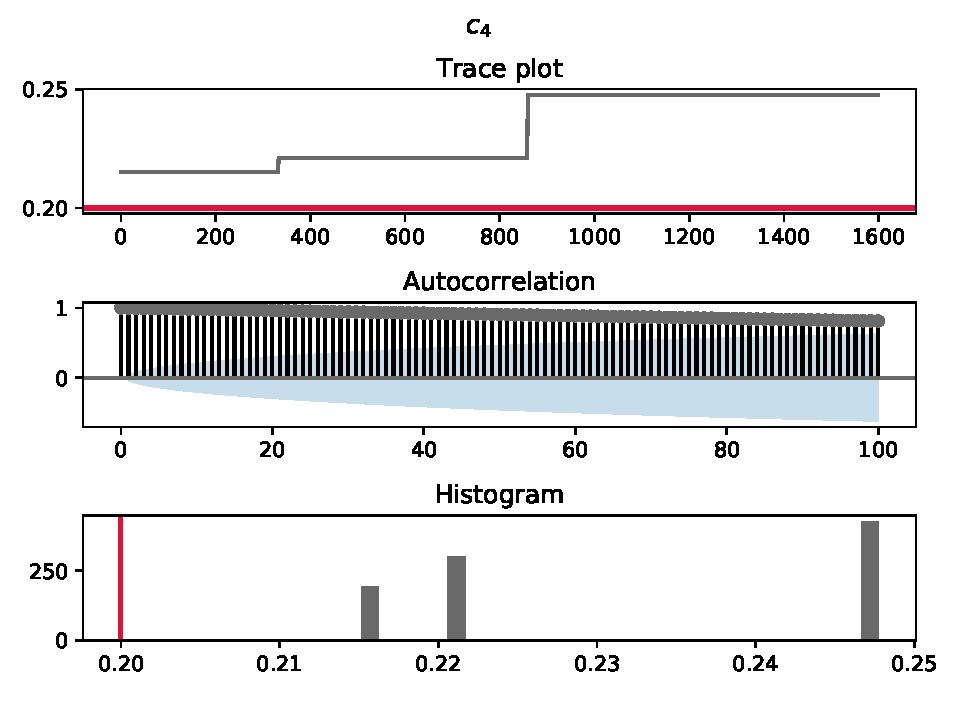
\includegraphics[width=0.45\textwidth]{autoregulation/pmh_cauchy_c4} }}%
    \caption{Particle filter-based inference of the parameters $c_3$ and $c_4$ in the auto-regulation model. Uses Cauchy noise and a Gaussian observation model. The true values are shown in red.}%
    \label{fig:ar-pmh-cauchy-2}%
\end{figure}

\begin{figure}[htp]%
    \centering
    \subfloat[$c_7$]{{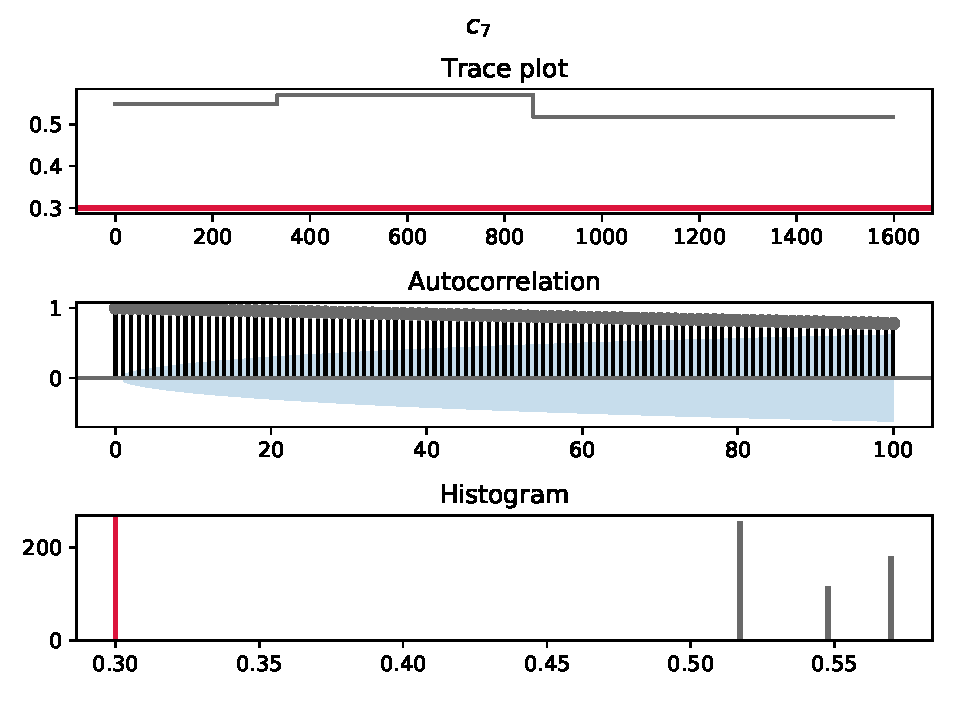
\includegraphics[width=0.45\textwidth]{autoregulation/pmh_cauchy_c7} }}%
    \qquad
    \subfloat[$c_8$]{{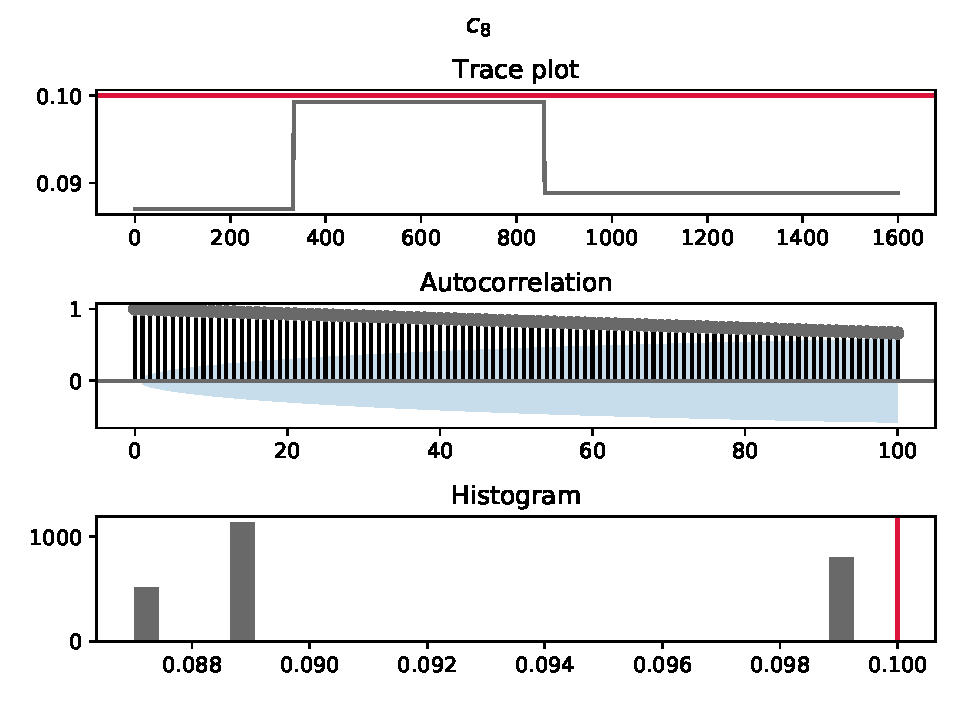
\includegraphics[width=0.45\textwidth]{autoregulation/pmh_cauchy_c8} }}%
    \caption{Particle filter-based inference of the parameters $c_7$ and $c_8$ in the auto-regulation model. Uses Cauchy noise and a Gaussian observation model. The true values are shown in red.}%
    \label{fig:ar-pmh-cauchy-3}%
\end{figure}


\subsection{Inference using ABC}
Next, we apply the marginal Metropolis-Hastings algorithm depending on the ABC methods.

\paragraph{Gaussian noise, Gaussian kernel}
At first, we use an input sequence corrupted by a Gaussian noise, as described above, and use ABC with a Gaussian kernel. The results are shown in \autoref{fig:ar-abcmh-gauss-gauss-1}, \autoref{fig:ar-abcmh-gauss-gauss-2} and \autoref{fig:ar-abcmh-gauss-gauss-3}.

Unfortunately, it appears that the ABC approximation introduces too much bias to the inference, as only two parameters ($c_4$ and $c_7$) are correctly identified. In addition, the samples for $c_8$ are not as far off, judging from the x-axis labels. Samples for the remaining parameters have diverged from the true values. As was the case with the particle filter, there is a strong autocorrelation present in the sampled values.

Some indications given in \cite{wilkinson-book} state that ABC (though applied in a different context than SSMs) together with the simple Gillespie algorithm can lead to poor results. To obtain better estimates, more sophisticated reaction simulators should be considered for the complex problems studied in molecular biology.

\begin{figure}[htp]%
    \centering
    \subfloat[$c_1$]{{\includegraphics[width=0.45\textwidth]{autoregulation/abcmh_gauss_gauss_c1} }}%
    \qquad
    \subfloat[$c_2$]{{\includegraphics[width=0.45\textwidth]{autoregulation/abcmh_gauss_gauss_c2} }}%
    \caption{ABC-based inference of the parameters $c_1$ and $c_2$ in the auto-regulation model. Uses Gaussian noise and a Gaussian kernel. The true values are shown in red.}%
    \label{fig:ar-abcmh-gauss-gauss-1}%
\end{figure}

\begin{figure}[htp]%
    \centering
    \subfloat[$c_3$]{{\includegraphics[width=0.45\textwidth]{autoregulation/abcmh_gauss_gauss_c3} }}%
    \qquad
    \subfloat[$c_4$]{{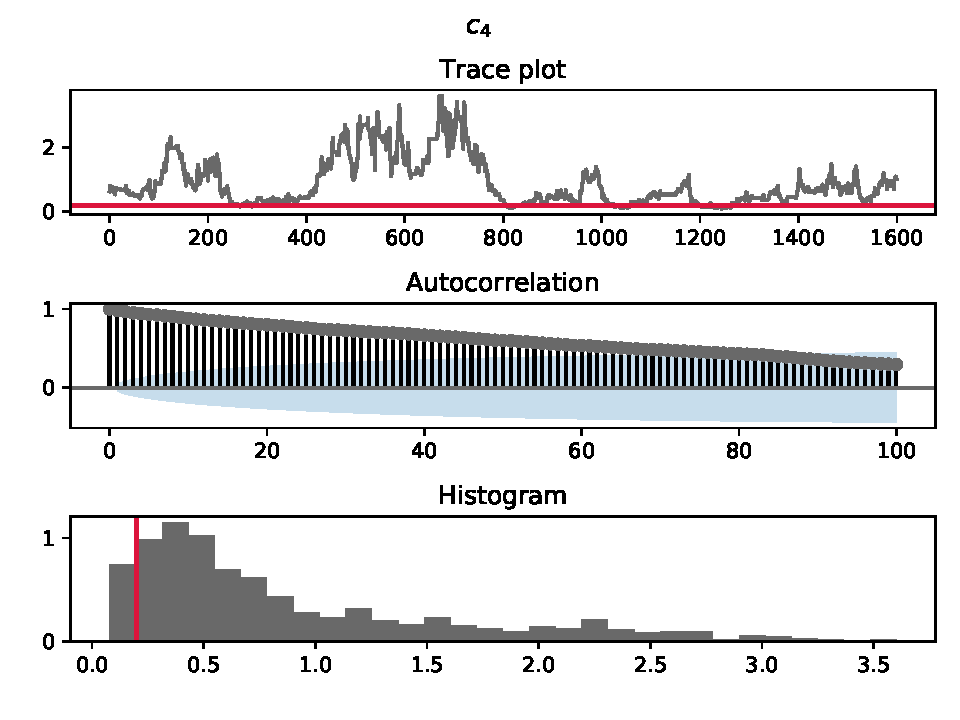
\includegraphics[width=0.45\textwidth]{autoregulation/abcmh_gauss_gauss_c4} }}%
    \caption{ABC-based inference of the parameters $c_3$ and $c_4$ in the auto-regulation model. Uses Gaussian noise and a Gaussian kernel. The true values are shown in red.}%
    \label{fig:ar-abcmh-gauss-gauss-2}%
\end{figure}

\begin{figure}[htp]%
    \centering
    \subfloat[$c_7$]{{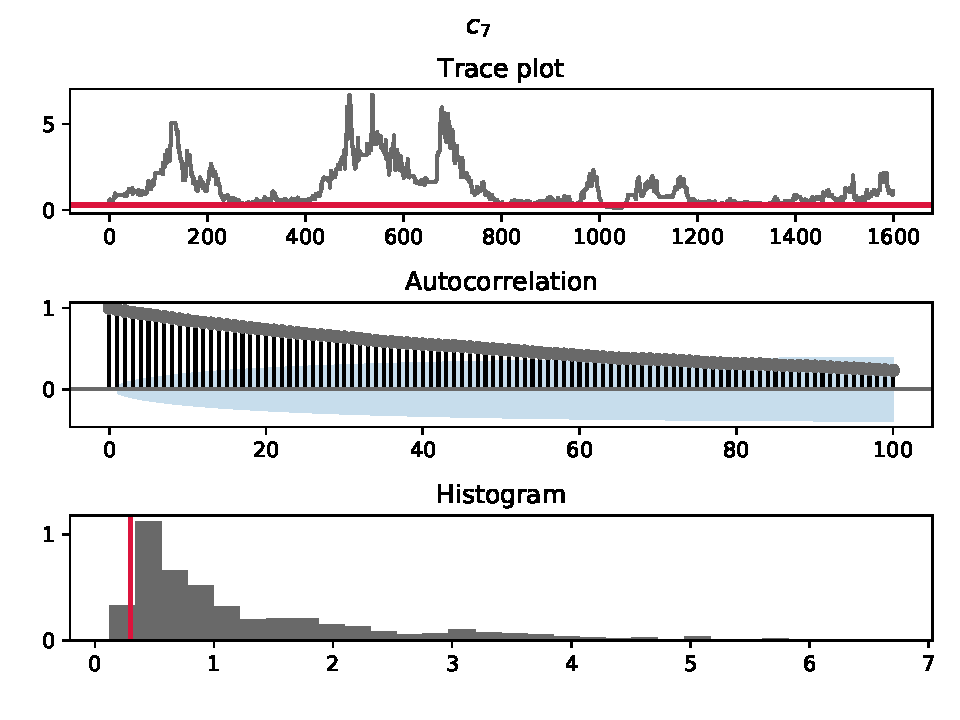
\includegraphics[width=0.45\textwidth]{autoregulation/abcmh_gauss_gauss_c7} }}%
    \qquad
    \subfloat[$c_8$]{{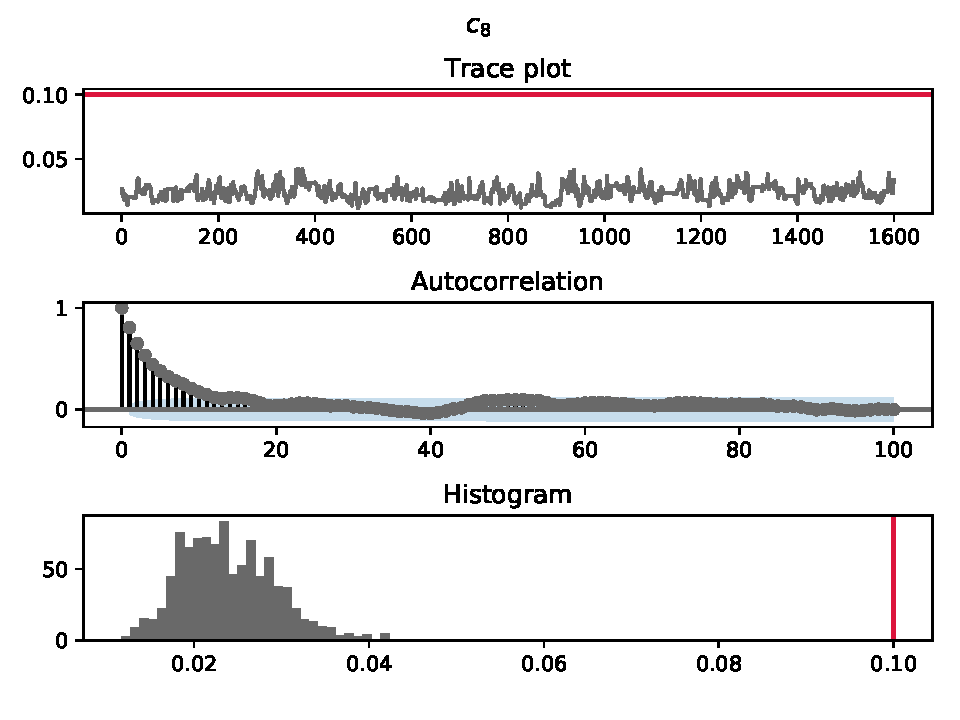
\includegraphics[width=0.45\textwidth]{autoregulation/abcmh_gauss_gauss_c8} }}%
    \caption{ABC-based inference of the parameters $c_7$ and $c_8$ in the auto-regulation model. Uses Gaussian noise and a Gaussian kernel. The true values are shown in red.}%
    \label{fig:ar-abcmh-gauss-gauss-3}%
\end{figure}


\paragraph{Cauchy noise, Gaussian kernel}
Next, we again apply the heavy-tailed Cauchy noise to the input sequence, but keep using the Gaussian kernel. We are interested to see whether the filter collapses, as was the case in particle filter-based inference under a misspecified model. The results are shown in \autoref{fig:ar-abcmh-cauchy-gauss-1}, \autoref{fig:ar-abcmh-cauchy-gauss-2} and \autoref{fig:ar-abcmh-cauchy-gauss-3}.

The situation is similar to the previous experiment with Gaussian noise. The parameters $c_1, c_4$ and to a lesser degree, $c_8$, are identified. The samples of the other parameters diverge.

Unlike the particle filter, our method again does not collapse under model misspecification. It is still a better choice if we do not have access to the correct model, as it manages to identify at least some parameters.

\begin{figure}[htp]%
    \centering
    \subfloat[$c_1$]{{\includegraphics[width=0.45\textwidth]{autoregulation/abcmh_cauchy_gauss_c1} }}%
    \qquad
    \subfloat[$c_2$]{{\includegraphics[width=0.45\textwidth]{autoregulation/abcmh_cauchy_gauss_c2} }}%
    \caption{ABC-based inference of the parameters $c_1$ and $c_2$ in the auto-regulation model. Uses Cauchy noise and a Gaussian kernel. The true values are shown in red.}%
    \label{fig:ar-abcmh-cauchy-gauss-1}%
\end{figure}

\begin{figure}[htp]%
    \centering
    \subfloat[$c_3$]{{\includegraphics[width=0.45\textwidth]{autoregulation/abcmh_cauchy_gauss_c3} }}%
    \qquad
    \subfloat[$c_4$]{{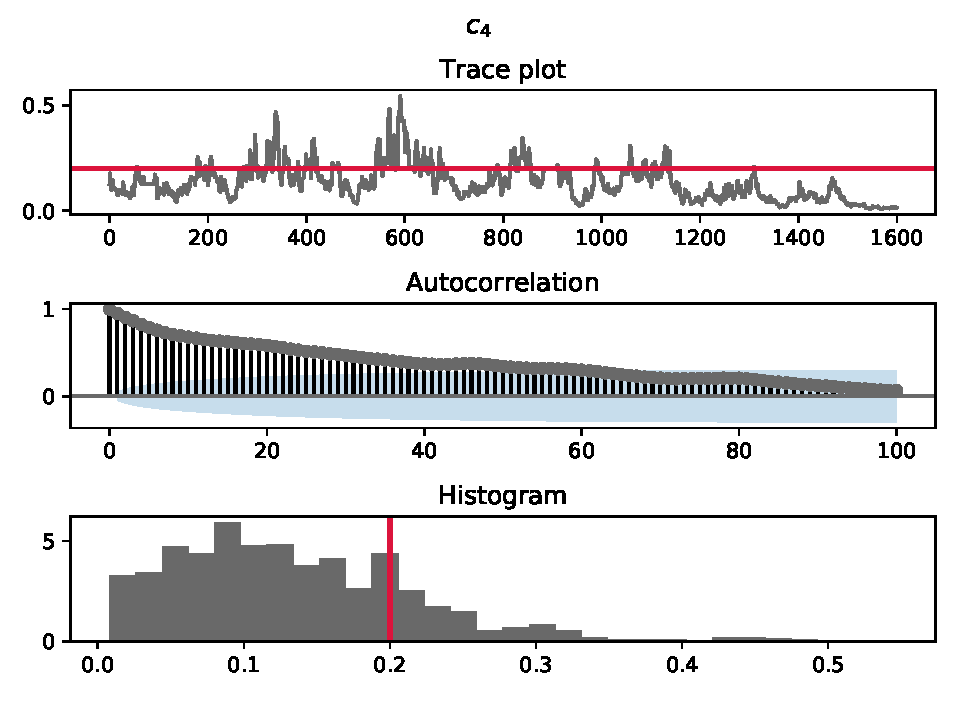
\includegraphics[width=0.45\textwidth]{autoregulation/abcmh_cauchy_gauss_c4} }}%
    \caption{ABC-based inference of the parameters $c_3$ and $c_4$ in the auto-regulation model. Uses Cauchy noise and a Gaussian kernel. The true values are shown in red.}%
    \label{fig:ar-abcmh-cauchy-gauss-2}%
\end{figure}

\begin{figure}[htp]%
    \centering
    \subfloat[$c_7$]{{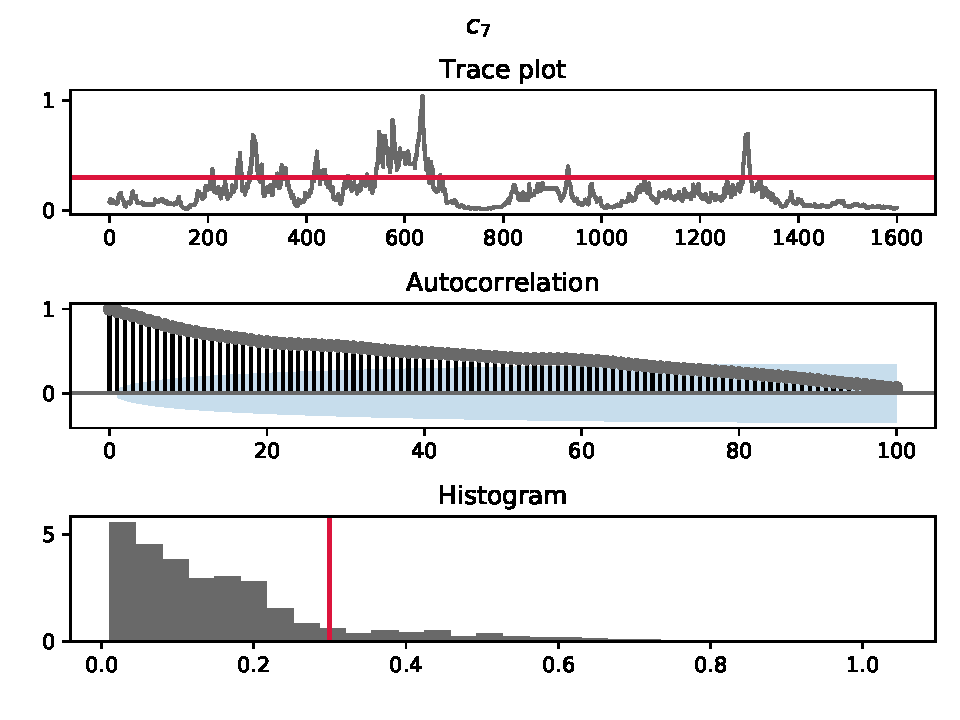
\includegraphics[width=0.45\textwidth]{autoregulation/abcmh_cauchy_gauss_c7} }}%
    \qquad
    \subfloat[$c_8$]{{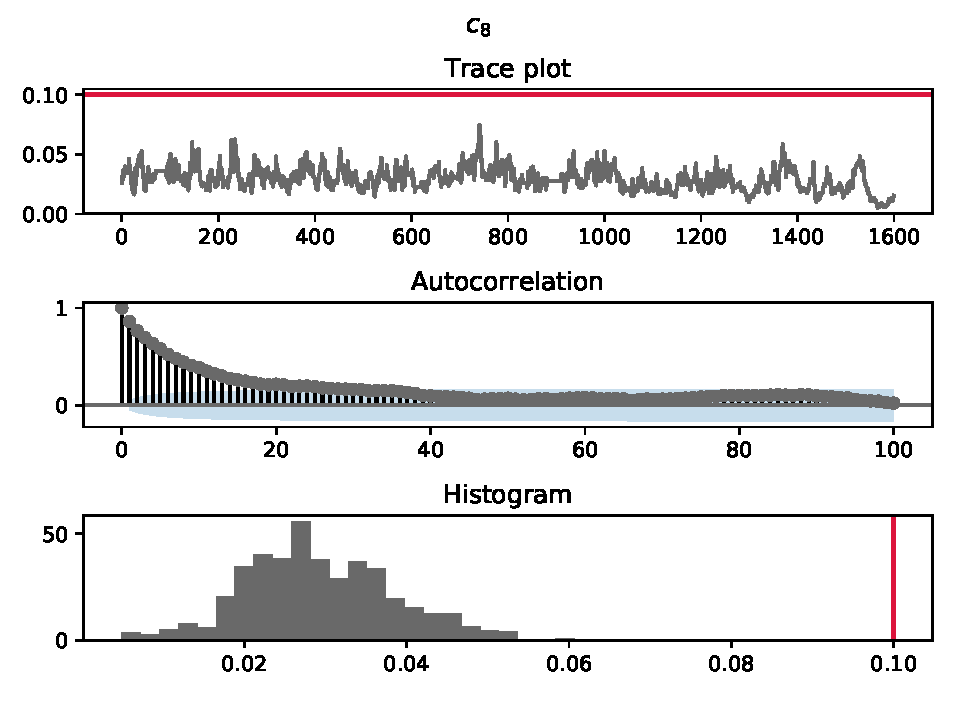
\includegraphics[width=0.45\textwidth]{autoregulation/abcmh_cauchy_gauss_c8} }}%
    \caption{ABC-based inference of the parameters $c_7$ and $c_8$ in the auto-regulation model. Uses Cauchy noise and a Gaussian kernel. The true values are shown in red.}%
    \label{fig:ar-abcmh-cauchy-gauss-3}%
\end{figure}

\paragraph{Cauchy noise, Cauchy kernel}
Finally, we are interested to see what happens when we keep the Cauchy noise on the input sequence but use the Cauchy kernel. The results are shown in \autoref{fig:ar-abcmh-cauchy-cauchy-1}, \autoref{fig:ar-abcmh-cauchy-cauchy-2} and \autoref{fig:ar-abcmh-cauchy-cauchy-3}.

As expected, the filter does not collapse. There is still a notable identification problem, similarly to the the previous two experiments -- a simple change in the kernel function cannot significantly improve the estimate quality. Compared to the Gaussian kernel experiment, the sampled values are somewhat more spread out.

\begin{figure}[htp]%
    \centering
    \subfloat[$c_1$]{{\includegraphics[width=0.45\textwidth]{autoregulation/abcmh_cauchy_cauchy_c1} }}%
    \qquad
    \subfloat[$c_2$]{{\includegraphics[width=0.45\textwidth]{autoregulation/abcmh_cauchy_cauchy_c2} }}%
    \caption{ABC-based inference of the parameters $c_1$ and $c_2$ in the auto-regulation model. Uses Cauchy noise and a Cauchy kernel. The true values are shown in red.}%
    \label{fig:ar-abcmh-cauchy-cauchy-1}%
\end{figure}

\begin{figure}[htp]%
    \centering
    \subfloat[$c_3$]{{\includegraphics[width=0.45\textwidth]{autoregulation/abcmh_cauchy_cauchy_c3} }}%
    \qquad
    \subfloat[$c_4$]{{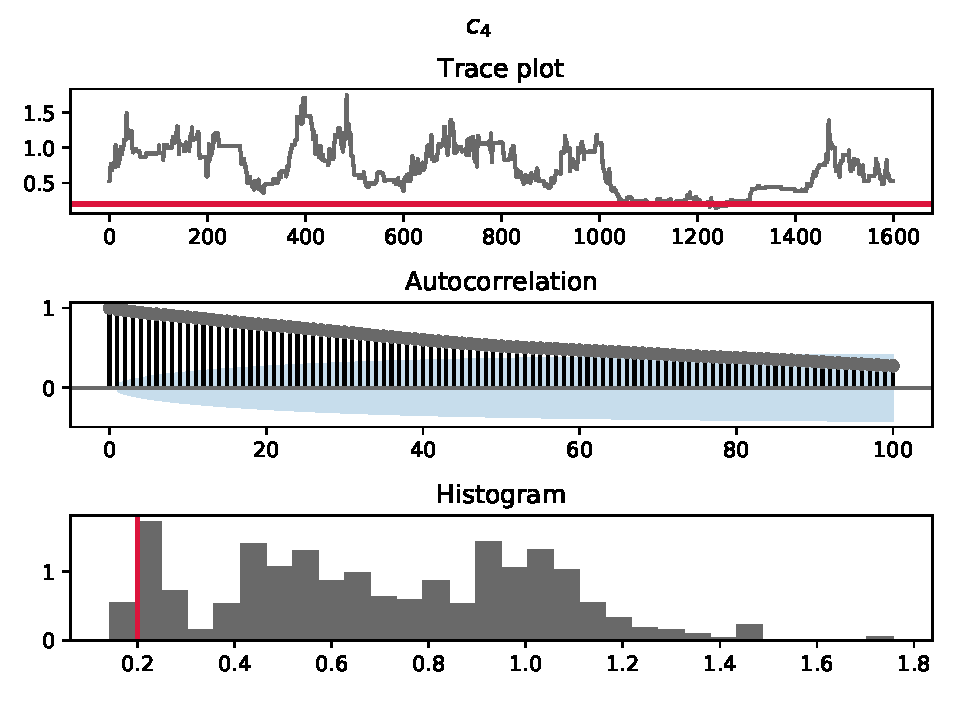
\includegraphics[width=0.45\textwidth]{autoregulation/abcmh_cauchy_cauchy_c4} }}%
    \caption{ABC-based inference of the parameters $c_3$ and $c_4$ in the auto-regulation model. Uses Cauchy noise and a Cauchy kernel. The true values are shown in red.}%
    \label{fig:ar-abcmh-cauchy-cauchy-2}%
\end{figure}

\begin{figure}[htp]%
    \centering
    \subfloat[$c_7$]{{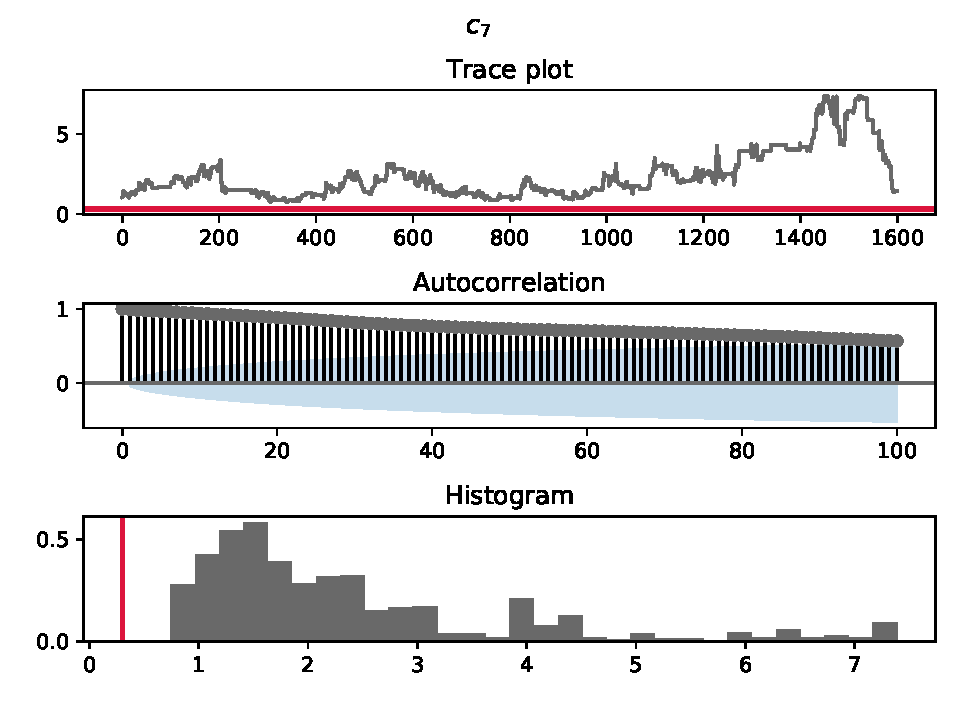
\includegraphics[width=0.45\textwidth]{autoregulation/abcmh_cauchy_cauchy_c7} }}%
    \qquad
    \subfloat[$c_8$]{{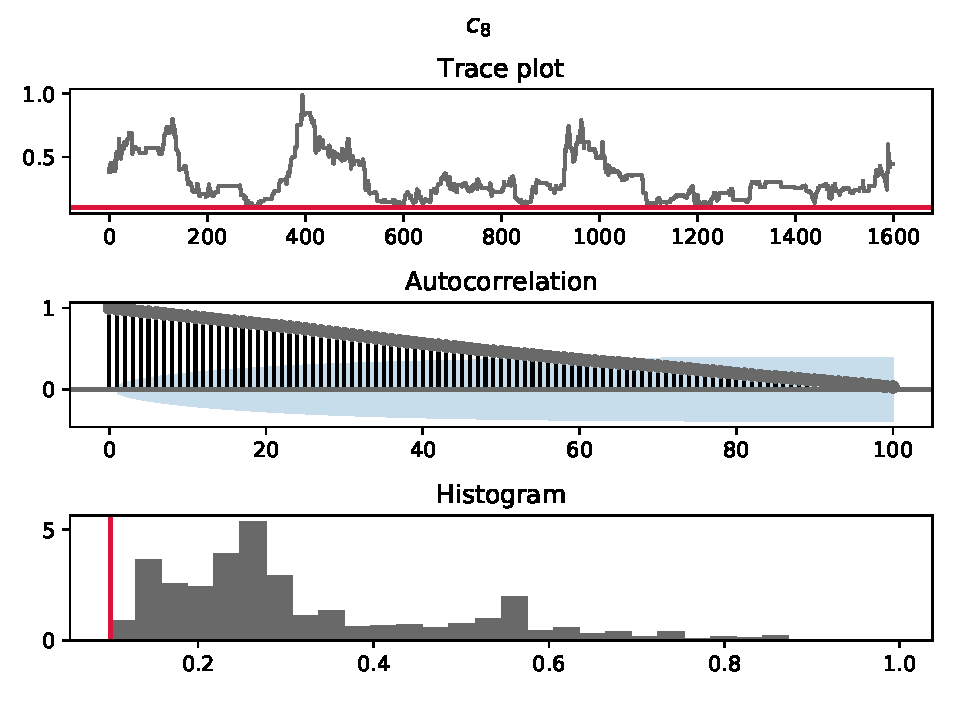
\includegraphics[width=0.45\textwidth]{autoregulation/abcmh_cauchy_cauchy_c8} }}%
    \caption{ABC-based inference of the parameters $c_7$ and $c_8$ in the auto-regulation model. Uses Cauchy noise and a Cauchy kernel. The true values are shown in red.}%
    \label{fig:ar-abcmh-cauchy-cauchy-3}%
\end{figure}


\subsection{Experiment conclusion}
We applied our model to a simplified model of a prokaryotic autoregulatory network. As in the Lotka-Volterra study, the latent spaces were again simulated using the Gillespie algorithm. In this experiment, inference was much more difficult, as the observed sequence $\by_t$ was only a one-dimensional linear combination of two of the four elements of the state vector $\bx_t$.

The particle filter under a correct observation model managed to identify the static parameter well. When this model was misspecified, the filter completely collapsed and the results became unusable, as was expected.

Our ABC-based method introduced too much bias and encountered identification problems in about half of the unknown parameters. Nevertheless, the ABC filter does not collapse even when applied to a sequence corrupted by heavy-tailed noise. A possible cause for the unsatisfactory results is the simple Gillespie algorithm. It is likely that using a more complex simulation mechanism would lead to better results; this is a possibility left for future work.
